% A simple polygon and the parity of ray crossings (drawn by hand).
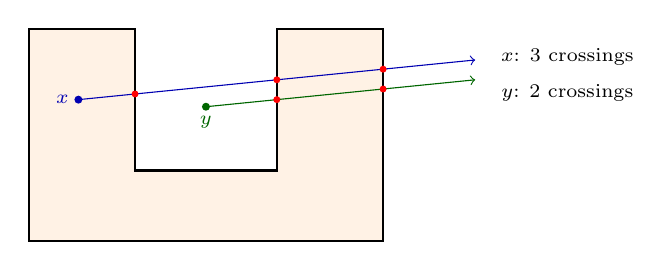
\begin{tikzpicture}[scale=0.9]
\fill[orange!10] (0,0)--(5,0)--(5,3)--(3.5,3)--(3.5,1)--(1.5,1)--(1.5,3)--(0,3)--cycle;
\draw[thick] (0,0)--(5,0)--(5,3)--(3.5,3)--(3.5,1)--(1.5,1)--(1.5,3)--(0,3)--cycle;
\draw[->,blue!70!black] (0.7,2)--(6.3,2.56);
\fill[blue!70!black] (0.7,2) circle (1.6pt) node[left,font=\scriptsize]{$x$};
\foreach \X/\Y in {1.5/2.08,3.5/2.28,5/2.43} \fill[red] (\X,\Y) circle (1.4pt);
\draw[->,green!40!black] (2.5,1.9)--(6.3,2.28);
\fill[green!40!black] (2.5,1.9) circle (1.6pt) node[below,font=\scriptsize]{$y$};
\foreach \X/\Y in {3.5/2.0,5/2.15} \fill[red] (\X,\Y) circle (1.4pt);
\node[font=\scriptsize,align=left] at (7.6,2.6) {$x$: 3 crossings};
\node[font=\scriptsize,align=left] at (7.6,2.1) {$y$: 2 crossings};
\end{tikzpicture}
